Determining the LET at the test location is essential and is a function of both particle type and energy. The T08 transfer line which transports the beam from the PS to CHARM features \textbf{a considerable amount of in-beam instrumentation} and monitoring units, along a large fraction of distance traveled by the \textbf{beam in air} (delimited by vacuum windows). The beam line is predominantly used for 24 GeV/c proton operation for which the compound material budget has very little effect on the beam quality for protons when delivered to the test facilities IRRAD and CHARM. The situation changes drastically when the transport of VHE ions through T08 is requested, for which the present material budget in the different non-vacuum regions affects the beam quality through:
\begin{itemize}
    \item \textbf{Electronic stopping power} (dE/dx): Interaction of the beam particle charge with the electronic structure inside material results in a loss of particle kinetic energy, generally quantified by the Bethe formula \cite{Bethe30}, according to which, the average stopping power is proportional to the ratio of the target atomic and mass numbers Z$_T$ and A$_T$ and the density $\rho_T$:
\begin{equation}\label{stopping}
    dE/dx \propto \frac{Z_T}{A_T}\rho_T;
    \end{equation}
    Particles sourced with a fixed energy are subject to energy straggling, i.e. fluctuations in energy loss caused by the statistical nature of energy loss processes for charged particles in matter. A spread-out energy distribution around the mean given by the Bethe formula is inevitable after traversing material.
    \item \textbf{Inelastic interactions}: The beam particles have sufficient energy for triggering nuclear reactions with any material it crosses \cite{Lannunziata16}. The macroscopic cross section is proportional to the target material density $\rho_T$:

    \begin{equation}
    \sigma \propto \rho_T,
    \end{equation}
The microscopic cross section $\sigma$ for a reaction between a projectile and target can be approximated in a geometrical sense to first-order approximation \cite{Krane88}:  $\sigma = \pi (R_T + R_P)^2$   with the nuclear radius given by $R \propto A^{1/3}$.
    Evidently, when the beam crosses e.g. vacuum windows, a primary particle can be lost in a nuclear reaction and only secondary fragments remain. Due to the high beam energy and by consequence high velocity they will be transported predominantly in a forward fashion: this can cause considerable beam contamination of particles with different charge and energy; and by consequence different LET.
\end{itemize}

Both processes also affect the fluence: collisions with the electronic structure of materials causes angular scattering which spreads out the beam over larger surface areas; inelastic interactions deteriorate the amount of primary particles in the beam. The discussion of these effects are however out of the scope of this report.\\
\\
A suitable measure of the extent to which these two physics processes affect the beam characteristics is required. In the energy range under consideration, the stopping power exhibits a weak material dependency (due to the proportionality to Z/A). Hence, the material density and cumulative distance traveled through the material are the dominating factors. An effective, descriptive material property is the \emph{surface density} $l'$ which is the product of the material length $l$ and material density $\rho$:
\begin{equation}
l' = l \times \rho
\end{equation}
in units of [g/cm$^2$] and is commonly used when quantifying particle penetration in matter \cite{Lechner18}. We refer to the material or region length as the distance traveled within the material by an ideal beam particle. The surface density is also useful to describe the prevalence of inelastic collisions inside materials.\\
\\
The mean free path of a given type of particle and corresponding energy inside a material is also called the \emph{inelastic scattering length} and is a function of the projectile type, projectile energy and target material properties such as atomic composition and density. To give an example in the scope of the T08 simulations: the inelastic scattering length for Pb ions extracted at 1 GeV/n in titanium is roughly 4 cm, whereas in air it is 60 m. These values are similar for lower extracted energies (down to 100s MeV/n) and were all taken from the standard FLUKA simulation output file.\\
\\
 The surface density values for all (non-vacuum) materials the beam sees along the transfer line can already shed some light into where primary beam energy straggling and fragmentation is prevalent. In Table \ref{tab:material}, all non-vacuum materials seen by the beam are listed, including the surface density in the final column. To highlight an example: the XION070 instrument features two stainless steel vacuum windows and a set of stainless steel foils. Each of these, despite their $\mu$m level thickness, has a comparable surface density as the argon gas that the instrument is filled with which has a longer length but a much lower density. One can also infer from the table that the \textbf{biggest effects can be expected in the different air sections} given that these reach the highest surface density values due to the long distance crossed by the beam. The cumulative surface density is 5.38 g/cm$^2$, of which 3.88  g/cm$^2$, i.e., 72\% is due to air. \\
 \\
 However, a more detailed measure can be made by \textbf{Monte Carlo (MC) calculations}. MC simulations are an essential tool to quantify the effects of transport along the beam line. They are a decisive tool when it comes to providing a more fundamental and in-depth description of the beam and radiation environment and also allow to run multiple configurations and related optimizations in parallel; both of which are often not available experimentally. The general purpose Monte Carlo code FLUKA \cite{Battistoni15, FlukaWeb} is a most suitable tool, regularly used in accelerator environments and extensively benchmarked on a microscopic level \cite{Ahdida22, Braun14, Battistoni07}. When discussing the different elements in the form of their FLUKA simulation model analog we will generally talk about \emph{regions}, i.e., segments of the geometry composed of a single material. All calculations in this study were carried out in FLUKA versions 4.2 and 4.3 with checks between the two versions for consistency.
 
\begin{table}[htp]
\scriptsize
\centering
\caption{Material budget table for the November 2022 T08 beam line configuration and the corresponding FLUKA simulation model. Only the non-vacuum regions and their parent elements are listed, as function of their distance from the DUT location (along the $s$-axis). The region thickness is expressed in [cm] except for very thin subcomponents of instruments such as electrode foils or vacuum covers for which the thickness is expressed in [$\mu$m]. The surface density expression in units of [0.1 g/cm$^2$] was chosen to ease the comparison between different regions. In addition, the cumulative non-vacuum length is quoted.}
\label{tab:material}
\begin{threeparttable}
\resizebox{\textwidth}{!}{%
\begin{tabular}{lllllllS}
\toprule
\toprule
 & & Element & Position  & Thickness & Material & Density & \multicolumn{1}{r}{Surface density}\\
 & & & [m] & [cm] &  & [g/cm$^3$] & [0.1~g/cm$^2$]  \\
 \toprule
 & & SOURCE (PS) \\
 \midrule
 \multirow{10}{*}{\rotatebox[origin=c]{90}{F61} $\begin{dcases*} \\ \\ \\ \\ \\ \\ \\ \\ \\ \end{dcases*}$} & 1. & PS vacuum window & 123.97 & 0.01 & Ti & 4.540 & .45 \\
 & & \multicolumn{1}{r}{Air section} & 123.97 & 30.0 & air & 1.293$\cdot$10$^{-3}$ & .39\\
 & 2. & BTV01 vacuum window & 123.25 & 0.01 & Ti & 4.540 & .45 \\
 & 3. & BCTF022 vacuum window & 113.37 & 0.02 & Al & 2.699 & .54\\ 
 & & \multicolumn{1}{r}{Air section} & 113.37 & 17.7 & air & 1.293$\cdot$10$^{-3}$ & .23\\
 & 4. & BCGAA23 & 113.09 & $2\times 50 \mu$m & Al & 2.699 & .27 \\
 & & (Gaseous scint.) & & 6 & N$_2$ & 1.17$\cdot$10$^{-3}$ & .07 \\
 & & \multicolumn{1}{r}{Air section} & 113.09 & 4.0 & air & 1.293$\cdot$10$^{-3}$ & .05\\
 & 5. & XSEC023 & 112.81 & $2\times25 \mu$m & stainless steel & 7.9 & .40\\
 & & & & $2\times5\times5 \mu$m & Al & 2.699 & .13 \\
 & & \multicolumn{1}{r}{Air section} & 109.89 & 250.0 & air & 1.293$\cdot$10$^{-3}$ & 3.23\\
 & 6. & T08 vacuum window & 107.30 & 0.02 & Ti & 4.540 & .91 \\
 \\
 \multirow{9}{*}{\rotatebox[origin=c]{90}{T08} $\begin{dcases*} \\ \\ \\ \\ \\ \\ \\ \end{dcases*}$} & 7. & T08 vacuum window & 34.0 & 0.02 & Al & 2.699 & 0.54\\
 & & \multicolumn{1}{r}{Air section} & 34.00 & 15.0 & air & 1.293$\cdot$10$^{-3}$ & 0.19\\
 & 8. & XSEC070 & 33.80 & $2\times25 \mu$m & stainless steel & 7.9 & 0.40\\
 & & & & $21\times5 \mu$m & Al & 2.699 & 0.28\\
 & & \multicolumn{1}{r}{Air section} & 33.56 & 10.0 & air & 1.293$\cdot$10$^{-3}$ & 0.13\\
 & 9. & XION071 & 33.46 & $2\times25 \mu$m & stainless steel & 7.9 & 0.40\\
 & & & & $21\times5 \mu$m & Al & 2.699 & 0.28 \\
 & & & & 24.0 & Ar & 1.66$\cdot$10$^{-3}$ & 0.40 \\
 & & \multicolumn{1}{r}{Air section} & 33.22 & 75 & air & 1.293$\cdot$10$^{-3}$ & 0.97\\
 \\
 \multirow{16}{*}{\rotatebox[origin=c]{90}{IRRAD} $\begin{dcases*} \\ \\ \\ \\ \\ \\ \\ \\ \\ \\ \\ \\ \\ \end{dcases*}$} & 10. & BPM1 & 32.48 & 0.1 & Cu & 8.96 & 0.90\\
 & & & & 0.069 & Kapton & 1.42 & 0.98\\
 & 11. & IRRAD vacuum window & 32.48 & 0.02 & Al & 2.699 & 0.54\\
 & 12. & IRRAD vacuum window & 28.98 & 0.02 & Al & 2.699 & 0.54\\
 & & \multicolumn{1}{r}{Air section} & 28.98 & 411.0 & air & 1.293$\cdot$10$^{-3}$ & 5.31\\
 & 13. & BPM2 & 24.87 & 0.1 & Cu & 8.96 & 0.90\\
 & & & & 0.069 & Kapton & 1.42 & 0.98\\
 & & \multicolumn{1}{r}{Air section} & 24.87 & 174.0 & air & 1.293$\cdot$10$^{-3}$ & 2.25\\
 & 14. & XSCI & 23.13 & 0.028 & plastic scint. & 1.032 & 0.29\\
 & & \multicolumn{1}{r}{Air section} & 23.1 & 556.0 & air & 1.293$\cdot$10$^{-3}$ & 7.19\\
 & 15. & BPM3 & 17.54 & 0.1 & Cu & 8.96 & 0.90\\
 & & & & 0.069 & Kapton & 1.42 & 0.98\\
 & & \multicolumn{1}{r}{Air section} & 17.54 & 483.0 & air & 1.293$\cdot$10$^{-3}$ & 6.25\\
 & 16 & BPM4 & 12.71 & 0.1 & Cu & 8.96 & 0.90\\
 & & & & 0.069 & Kapton & 1.42 & 0.98\\
 & 17. & IRRAD vacuum window & 12.71 & 0.02 & Al & 2.699 & 0.54 \\
 & 18. & IRRAD vacuum window & 10.00 & 0.02 & Al & 2.699 & 0.54\\
 \\
 \multirow{8}{*}{\rotatebox[origin=c]{90}{CHARM} $\begin{dcases*} \\ \\ \\ \\ \\ \\ \end{dcases*}$}& & \multicolumn{1}{r}{Air section} & 10.00 & 8.0 & air & 1.293$\cdot$10$^{-3}$ & 0.10\\
 & 19. & XION094 & 9.92 & $2\times25 \mu$m & stainless steel & 7.9 & 0.40 \\
 & & & & $21\times5 \mu$m & Al & 2.699 & 0.28\\
 & & & & 24.0 & Ar & 1.66$\cdot$10$^{-3}$ & 0.40\\
 & & \multicolumn{1}{r}{Air section} & 9.68 & 10.0 & air & 1.293$\cdot$10$^{-3}$ & 0.13\\
 & 20. & XSEC094 & 9.58 & $2\times25 \mu$m & stainless steel & 7.9 & 0.40\\
 & & & & $5\times5 \mu$m & Al & 2.699 & 0.07\\
 & & \multicolumn{1}{r}{Air section} & 9.34 & 934.0 & air & 1.293$\cdot$10$^{-3}$ & 12.08\\
 \bottomrule
 & & DUT (CHARM) \\
\bottomrule
& & \textbf{Cumulative:} & & \textbf{30.83 m} & & & \multicolumn{1}{l}{\textbf{5.36 g/cm$^2$}}\\
\bottomrule
\bottomrule
\end{tabular}
}
\end{threeparttable}
\end{table}
%All:  7.12 + 3.59 + 29.17 + 13.68 = 53.56
%Air: 38.76
\subsection{Geometric model of the T08 beam line}


\begin{figure}[t]
    \centering
    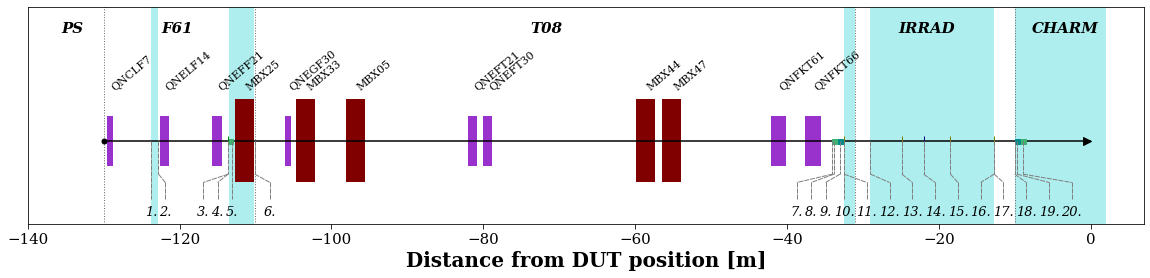
\includegraphics[width=\textwidth]{images/schematic.png}
    \vspace*{-0.5cm}
    \caption{Schematic representation of the T08 beam line, showing the main elements between the PS extraction point and test location in CHARM. The distance from the test location is measured along the $s$-axis of the beam reference frame. The beam line is subidivided in different zones: particles are extracted from the PS into the F61 before transported through the T08 line to experimental facilities IRRAD and ultimately CHARM. Optics elements such as bending dipole magnets (dark red) and quadrupole magnets (purple) are shown, along with the sections where the beam travels in air (cyan). The in-beam instrumentation units and vacuum windows are indicated and numbered according to Table \ref{tab:material}.}
    \label{fig:schematic}
\end{figure}

\begin{figure}[b]
    \centering
    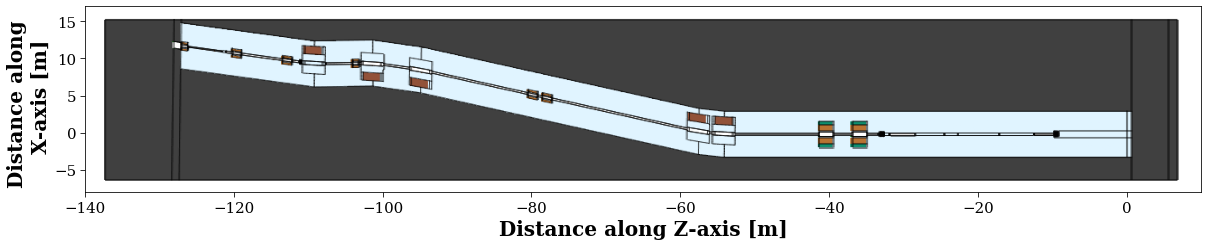
\includegraphics[width=\textwidth]{images/FLUKA_geometry.png}
    \vspace*{-0.5cm}
    \caption{Snapshot of the FLUKA geometry in the $xz$-plane as visualised in Flair \cite{Vlachoudis09}.}
    \label{fig:snapshot}
\end{figure}

In this report, the T08 beam line is described from the extraction point in the PS down to the \emph{device-under-test} (DUT) location in CHARM. By accelerator physics convention, we define the reference frame of the beam using the $s$-coordinate, which follows the beam along its ideal trajectory through the transfer line; the associated transverse coordinates $x$ and $y$ are of little relevance in this report. A schematic representation of the beam line is shown in Fig. \ref{fig:schematic}. The geometric model origin was chosen to be the DUT location in CHARM; its orientation was chosen such that the beam frame coincides with the geometric model frame in IRRAD and CHARM. The geometric model frame is spanned by the Cartesian $x$-, $y$- and $z$ axes, a snapshot of this geometry is shown in Fig. \ref{fig:snapshot}. \\
\\
As stated above, the goal of this study is to determine primary beam characteristics like the beam energy and associated LET. We are therefore only interested in accurately modeling direct interactions of the beam with the beam line infrastructure. The geometry was constructed using the LineBuilder python code \cite{Mereghetti12}, relying on the optics settings used during operation, dimensions from technical drawings and in-person inspections. The resulting model spans $\sim 140$ m from the PS extraction point to the chosen device-under-test (DUT) position located in the CHARM facility. The FLUKA model incorporates the correct materials, thicknesses (down to $\mu$m level) and respective distances for all elements the beam travels through. A complete description of the material budget seen by the beam is detailed in Table \ref{tab:material}, as it is implemented in the FLUKA model. We however restrict this detailed representation to the beam line aperture; outside, regions were assigned the FLUKA "black hole" material where particle tracking is killed upon entrance. This is also a necessary measure to keep the simulation time within limits, as will be further detailed in Section \ref{sec:physics} below.

\subsection{Physics and scoring settings}\label{sec:physics}
The particle source used in the FLUKA simulations was implemented as accurately as possible. The beam emittance and momentum spread were determined by measurements, serving as input to generate a phase space distribution with $x$, $x' (=dx/ds)$, $y$, $y'$ and $dp/p$ using \emph{pyBT}, a python package used by the Accelerator Beam Transfer group at CERN. The momentum dispersion  at extraction $dp/p_0$ is Gaussian shaped with a standard deviation that generally amounts to $\pm 0.3\%$. For each extracted kinetic energy, the $y$ and $y'$ were scaled by the relativistic factor $\beta \gamma$ to account the the fact that the beam gets larger when decelerated. From the generated initial distribution of 1M particles, 100K were randomly sampled to be simulated in FLUKA.\\
\\
The user-defined FLUKA simulation settings were chosen as a compromise between accuracy and simulation time: 
full transport of heavy ions (without any form of biasing) and hadronic particles down to 1 keV is necessary to track secondary fragments, neutrons are even transported down to 10$^{-5}$ eV which is the lowest limit. The generation of those fragments is accounted for by implying the appropriate heavy ion physics interaction models (such as electromagnetic dissociation). All other physics is properly handled by using the \emph{PRECISIOn} physics defaults. The interaction of heavy, charged particles with matter causes the production of particles in the electromagnetic sector (photons, electrons, positrons) through Bremsstrahlung and pair production processes. These particles are produced in large quantities and have longer ranges than the primary ions, potentially triggering other reactions. Since we are only interested in the energy loss and fragmentation of the primary particles, electromagnetic particles were dumped on the spot, depositing their full energy without transport, saving a considerable amount of computational resources.\\
 \\
Simulation data was extracted from the simulations by requesting dedicated information such as particle type, position, direction and total energy or momentum each time a particle crosses from any region in the geometric model to the next one. A dummy region was created to score the quantities exactly at the DUT position. This was done either by compiling the FLUKA executable with a dedicated user routine called \emph{mgdraw.f}, or using the \emph{USRYIELD} card which scores a double-differential particle yield, generally calculated with respect to physical quantities particle charge, energy or LET. The formatted output could be easily post-processed for analysis.

\subsection{Beam properties from simulation}
This section of the report is divided in two parts: first, we focus on the primary beam properties such as energy straggling, the resulting beam energy and LET (subsection \ref{sec:primary}). Second, the secondary particle distribution present at the DUT position is discussed (subsection \ref{sec:distribution}). The simulations carried out served the purpose of preparation of the CHIMERA experimental campaign by selecting an adequate set of energies and LETs. \textbf{The simulation results will be expressed as function of the final set of (extracted) kinetic energies: 650 MeV/n, 750 MeV/n and 1 GeV/n}. Each of these also has an official operational "username": CPS.USER.EAST4, CPS.USER.EAST3 and CPS.USER.MD5.  The quantities discussed in this section are summarized in Table \ref{tab:summary}.

\subsubsection{Primary beam properties at DUT position}\label{sec:primary}

\begin{figure}[b!]
    \centering
    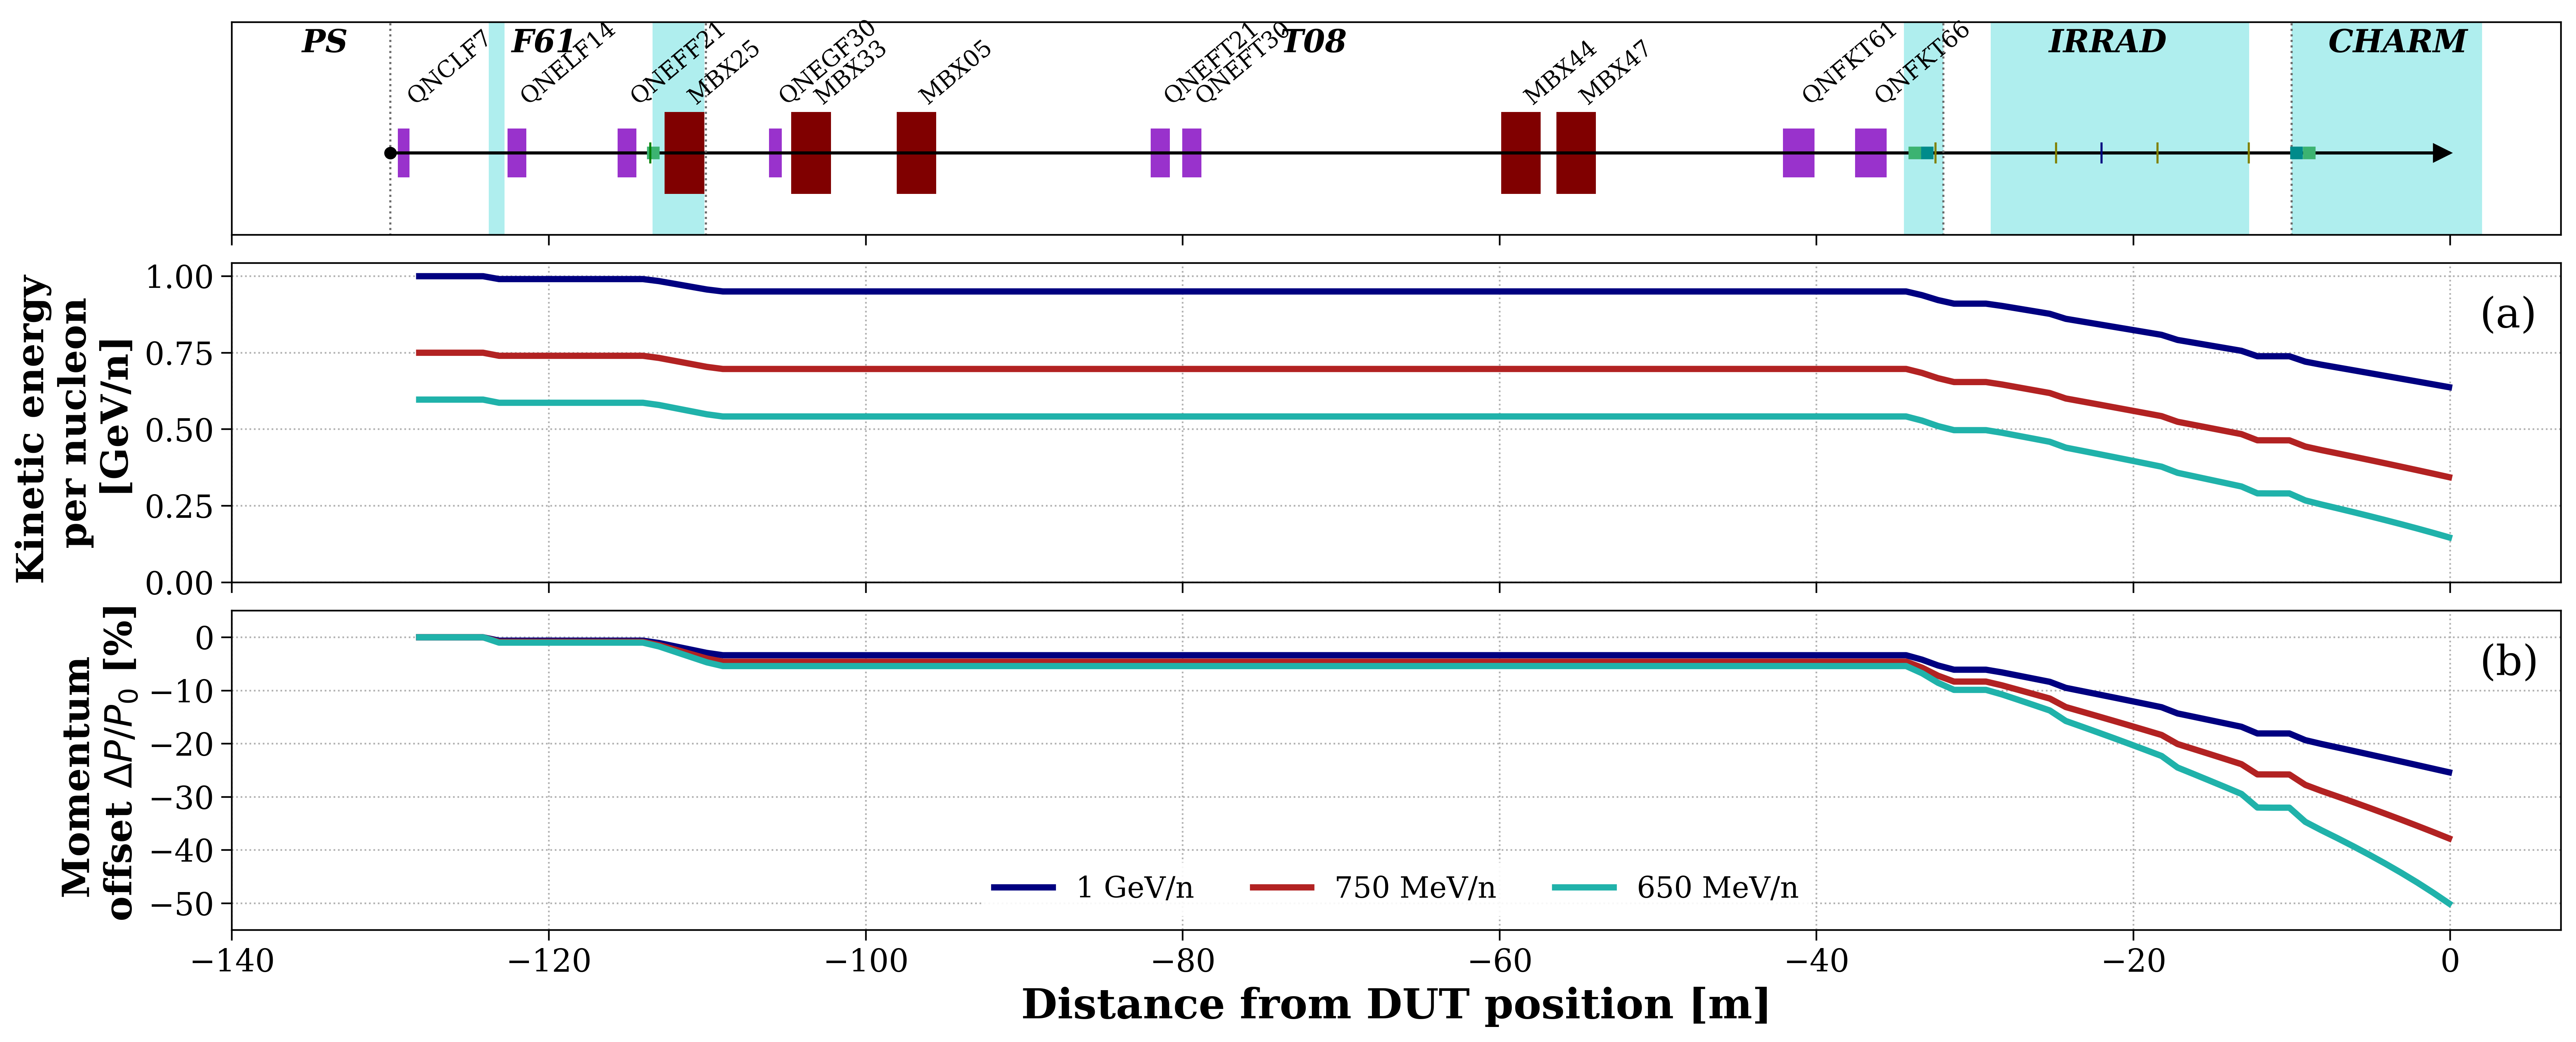
\includegraphics[width=\textwidth]{images/straggling.png}
    \vspace*{-0.5cm}
    \caption{FLUKA simulation results of the primary beam energy/momentum straggling for each of the energies used in the November 2022 experimental campaign, as function of the distance from the DUT position along the $s$-axis; shown for (a) the kinetic energy per nucleon, and (b) the momentum dispersion $\Delta P/P_0$ expressed in units of $[\%]$.}
    \label{fig:straggling_mean}
\end{figure}

As mentioned above, the primary Pb beam particles are sourced following a Gaussian momentum spread distribution with a $\pm 0.3\%$ standard deviation. E.g., at 1 GeV/n, a +0.3\% momentum offset amounts to a 5 MeV/n offset in kinetic energy per nucleon. Along the transfer line the momentum/energy distribution remains Gaussian, which for now we can disregard and focus on the mean. As shown in Fig. \ref{fig:straggling_mean}, it is clear that \textbf{the straggling is considerable and can be largely attributed to the IRRAD and CHARM experimental regions where the beam covers the largest distances in air}. The stopping power effect of the much denser materials present in the beam instrumentation and vacuum windows is obscured by the effect of the air since most of these elements are geometrically located inside these air sections (as also detailed in Table \ref{tab:material}). The kinetic energy per nucleon as function of distance from the DUT shown in Fig. \ref{fig:straggling} a) makes clear that the electronic stopping power due to the material budget has a qualitatively similar effect on all three primary energies in terms of energy loss with respect to the extracted primary energy. The 1 GeV/n beam is degraded down to 610 MeV/n, whereas the 650 MeV/n reaches down to 150 MeV/n. This has a profound effect on the associated LET which will be detailed further below. When expressed as momentum dispersion $\Delta P/P_0$ and shown in Fig. \ref{fig:straggling} b), it is clear that percentage-wise the lowest extracted energy is degraded the most: the 650 MeV/n kinetic energy beam loses over 50\% of its initial momentum.\\
\\
Given the long distance the beam travels through the transfer line and the presence of many non-vacuum sections, it is plausible that the primary beam energy/momentum spread is changed significantly. An initial Gaussian momentum distribution with a $\pm 0.3\%$ standard deviation may be spread out much more through successive interactions with materials. In what follows, we will express the distribution width in terms of the full width at half maximum, i.e. FWHM $\approx$ 2.355 $\sigma$. All primary beam energy distributions at the DUT are shown in Fig. \ref{fig:straggling}, including Gaussian fit parameters that show the mean and spread, the results are also summarized in Table \ref{tab:summary}. \textbf{For each extracted energy the FWHM of the distribution of primary beam particles is between 10 and 15 MeV/n}. This is not a big increase from the initial distribution spread which is also quoted in Table \ref{tab:summary}. \\
\\
For reference, we include the results of a simulation for 650 MeV/n extracted energy that is pencil-like; i.e., it has a fixed momentum and direction. The resulting distribution at the DUT position is indicative of a lower limit of spread which is inherent to the transfer line itself and amounts to slightly less than 1 MeV/n. The slightly lower mean value for the pencil beam is an effect of the beam line itself: the transmission of particles through the transfer line optics is affected by their particular momentum offset.

\begin{figure}[t!]
    \centering
    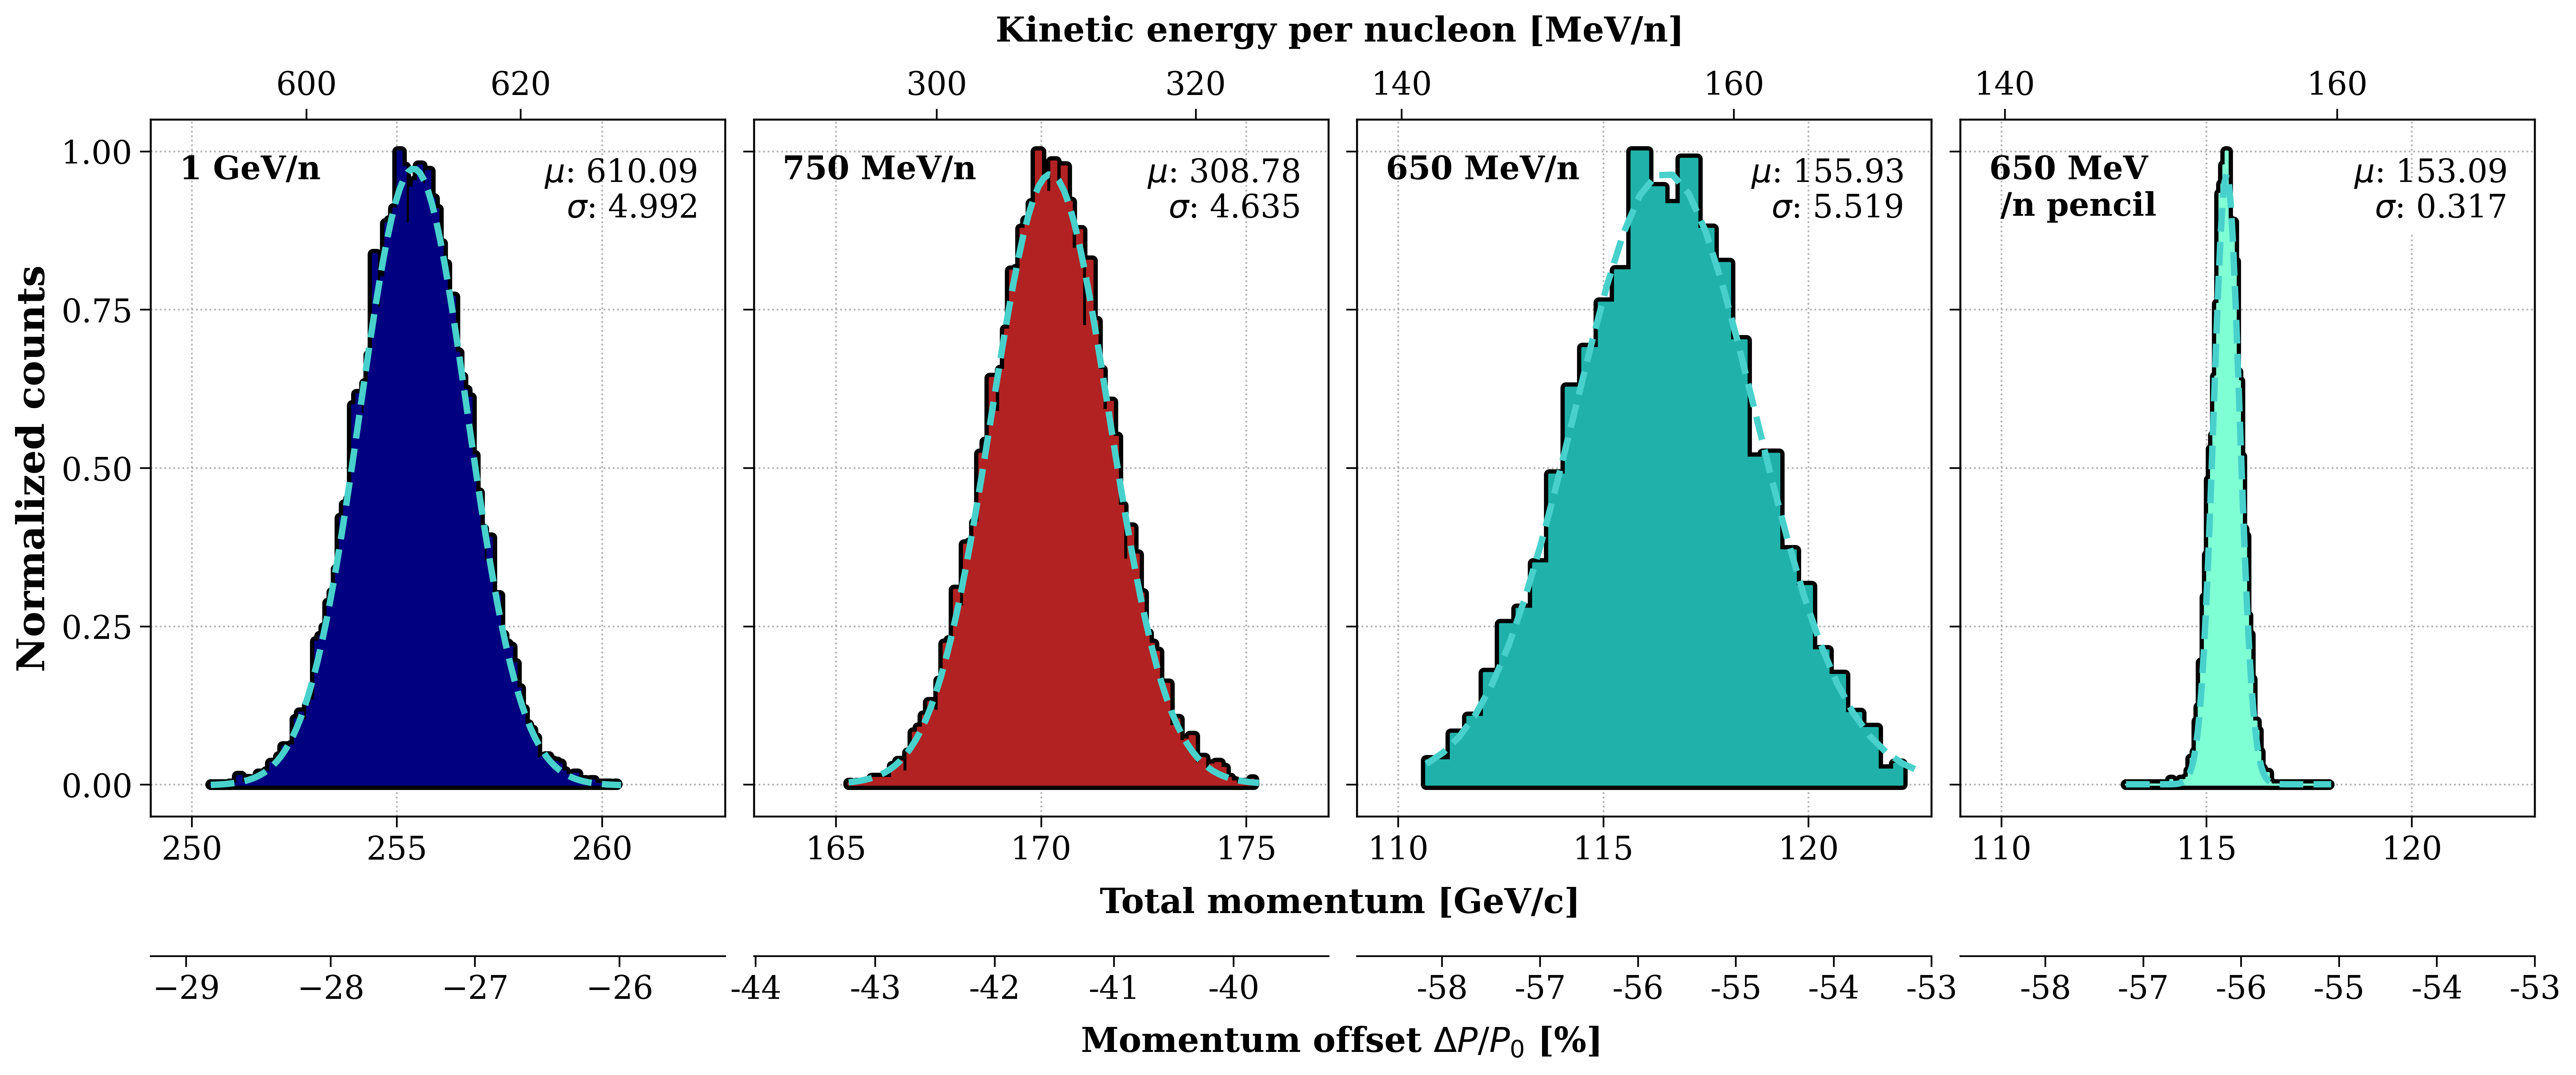
\includegraphics[width=\textwidth]{images/Resulting_energies.png}
    \vspace*{-0.5cm}
    \caption{FLUKA simulation results of the primary beam kinetic energy/momentum at the DUT position for each of the energies used in the November 2022 experimental campaign. Gaussian fit parameters are expressed in kinetic energy per nucleon [MeV/n]. The bottom axes express the beam parameters in terms of momentum and momentum offset. In addition, for 650 MeV/n the resulting distribution when using a pencil beam (fixed direction and momentum) is shown.}
    \label{fig:straggling}
\end{figure}


\begin{table}[h!]
   \scriptsize
    \centering
    \caption{Beam parameters subdivided between properties in the PS and at the DUT location. The properties in the PS also represent the FLUKA simulation initial conditions. For all quantities that were calculated from a distribution, the  mean and FWHM (in parentheses below) are quoted. The values for the pencil 650 MeV/n beam are only shown where applicable. From the simulations, we can assume a $\pm$ 1 MeVcm$^2$/mg error on the LET at the DUT location.}
    %\resizebox{\textwidth}{!}{%
    \label{tab:summary}
    \resizebox{\textwidth}{!}{%
    \begin{tabular}{c|rc|ccc||c|}
    \hline
    \hline
    & \multirow{2}{*}{USER} &&  CPS.USER & CPS.USER & CPS.USER & 650 MeV/n \\
    & && .EAST4 & .EAST3 & .MD5 & pencil \\
    \hline
    \multicolumn{1}{|c|}{\multirow{7}{*}{\rotatebox[origin=c]{90}{\makecell{EXTRACTED \\ FROM PS}}}} & & & & & & \\
    \multicolumn{1}{|c|}{} & Total momentum & & 351.92 & 291.15 & 265.79 & 265.79 \\
    \multicolumn{1}{|c|}{} & {[GeV/c]} &  & (2.47) & (2.04) & (1.86) & (0.0)  \\
    \multicolumn{1}{|c|}{} & & & & & & \\
    \multicolumn{1}{|c|}{} & Kinetic energy & & \textbf{1000.0} & \textbf{750.0} & \textbf{650.0} & 650.0 \\
     \multicolumn{1}{|c|}{}&  per nucleon [MeV/n]&  & (10.51) & (8.20) & (7.12) & (0.0)\\
      \multicolumn{1}{|c|}{} & & & & & & \\
      \hline
       \multicolumn{1}{c}{}\\
       \multicolumn{1}{c}{}\\
      \hline
    \multicolumn{1}{|c|}{\multirow{30}{*}{\rotatebox[origin=c]{90}{\makecell{AT CHARM \\ DUT LOCATION}}}} & & & & & & \\
        \multicolumn{1}{|c|}{} & Total momentum & & 255.46 & 170.31 & 116.69 & 115.54 \\
    \multicolumn{1}{|c|}{} & {[GeV/c]} & & (3.04) & (3.40) & (5.16) & (0.74) \\
    \multicolumn{1}{|c|}{} & & & & & & \\
    \multicolumn{1}{|c|}{} & Momentum offset & & 27.41 & 41.50 & 56.10 & 56.53 \\
    \multicolumn{1}{|c|}{} & $\Delta P/P_0$ [\%] & & (0.86) & (1.17) & (1.94) & (0.56) \\
    \multicolumn{1}{|c|}{} & & & & & & \\
    \multicolumn{1}{|c|}{} & Kinetic energy per nucleon & &\textbf{610.09} & \textbf{308.78} & \textbf{155.93} & 153.09\\
    \multicolumn{1}{|c|}{} & [MeV/n] & & (11.76) & (10.92) & (13.00) & (0.75) \\
    \multicolumn{1}{|c|}{} & & & & & &\\
    \multicolumn{1}{|c|}{} & & & & & &\\
    \multicolumn{1}{|c|}{} & \multirow{4}{*}{\makecell[r]{LET \\ {[MeVcm$^2$/mg]}}} & \multicolumn{1}{|c|}{\multirow{2}{*}{FLUKA}} & \textbf{13.42} & \textbf{18.40} & \textbf{26.53} & 26.83 \\
    \multicolumn{1}{|c|}{} & & \multicolumn{1}{|c|}{} & (0.10) & (0.32) & (1.33) & (0.19) \\
    \multicolumn{1}{|c|}{} & &\multicolumn{1}{|c|}{} & & & & \\
    \multicolumn{1}{|c|}{} & & \multicolumn{1}{|c|}{SRIM} & 13.43 & 17.77 & 25.67 & 25.95 \\
    \multicolumn{1}{|c|}{} & &  & & & & \\
    \multicolumn{1}{|c|}{} & &  & & & & \\
    \multicolumn{1}{|c|}{} & \multirow{3}{*}{\makecell[r]{Range (SRIM) \\ {[mm]}}} &\multicolumn{1}{|c|}{Si} & 28.73 & 10.12 & 3.95 & \\
    \multicolumn{1}{|c|}{} & & \multicolumn{1}{|c|}{}  & & & & \\
    \multicolumn{1}{|c|}{} & & \multicolumn{1}{|c|}{PMMA} & 45.71 & 16.36 & 5.61 &  \\
    \multicolumn{1}{|c|}{} & & & & & & \\
    \multicolumn{1}{|c|}{} & &  & & & & \\
    \multicolumn{1}{|c|}{} & \multirow{3}{*}{\makecell[r]{Energy deposition in \\300 $\mu$m of Si {[MeV]}}} &\multicolumn{1}{|c|}{FLUKA LET} & 938.06 & 1286.16 & 1854.45 & \\
    \multicolumn{1}{|c|}{} & & \multicolumn{1}{|c|}{}  & & & & \\
    \multicolumn{1}{|c|}{} & &\multicolumn{1}{|c|}{SRIM LET} & 938.76 & 1242.12 & 1794.33 & \\
    \multicolumn{1}{|c|}{} & & & & & & \\
    \multicolumn{1}{|c|}{} & &  & & & & \\
    \multicolumn{1}{|c|}{} & Fragmentation ratio & & \multirow{2}{*}{62.64} & \multirow{2}{*}{62.30} & \multirow{2}{*}{64.63} &\\
    \multicolumn{1}{|c|}{} & (Primary ions/total ions) [\%] & & & & &\\
    \multicolumn{1}{|c|}{} & &  & & & & \\
    \hline
    \hline
    
 \end{tabular}
    }
\end{table}


\subsubsection{Fragmentation and distributions at DUT positions}\label{sec:distribution}

As already introduced above, inelastic collisions of the primary beam particles with in-beam material inevitably causes the generation of secondary fragments. The large primary beam energy causes these fragments to travel along the beam and potentially arrive at the DUT testing location as well. This is visualised in Fig. \ref{fig:fragmentation} which shows that for all primary beams we get a continuous distribution in both energy per nucleon as atomic number Z. The distributions extend from zero up to the degraded primary beam energy (as shown in Fig. \ref{fig:straggling} and up to the Pb atomic number 82, showing that within these limits \textbf{we can expect a large variety of fragments at the DUT location}. For each of the extracted primary beams, a little over \textbf{a third of the particles arriving to the DUT location is a secondary fragment}. This is also summarized in Table \ref{tab:summary} as the ratio between primary beam ions and all ions arriving to the DUT.\\
\\
As result of these interactions, the particle energy, mass and charge can be altered which results in a different LET value. A full simulation taking into account both primary and secondary fragments is required to determine the LET distribution at the DUT location. This is shown in Fig. \ref{fig:LET} for each of the primary energies, where in each case a primary peak is accompanied by a tail of lower LET values. In the 1 GeV/n case, the modulation by the fragment atomic number is clearly visible: this is caused by the projectile-like fragments that are generated have roughly the same energy as the primary beam particle but have a different atomic number. This directly affects the electronic stopping power due to its Z-dependence (Eq. \ref{stopping}). The primary peaks were fitted with Gaussian functions to determine the centroid LET value and the width of the primary peak; the fit values are listed in Table \ref{tab:summary}. As shown above, the absolute spread of the primary kinetic energy distribution at the DUT is not drastically different between the three primary extracted values. \textbf{By consequence,  the LET spread is also limited, remaining well below 0.5 MeVcm$^2$/mg for the 1 GeV/n and 750 MeV/n extracted energies. At lower energy, also the LET variability is bigger, this is why the the LET spread at 650 MeV/n is almost 1.5 MeVcm$^2$/mg.} Another clear example is that the primary beam LET spread for the 650 MeV/n pencil-like beam is twice as large as the primary LET spread for 1 GeV/n. These are all important considerations to take into account when estimating the expected SEE response during testing.

\begin{figure}[t!]
    \centering
    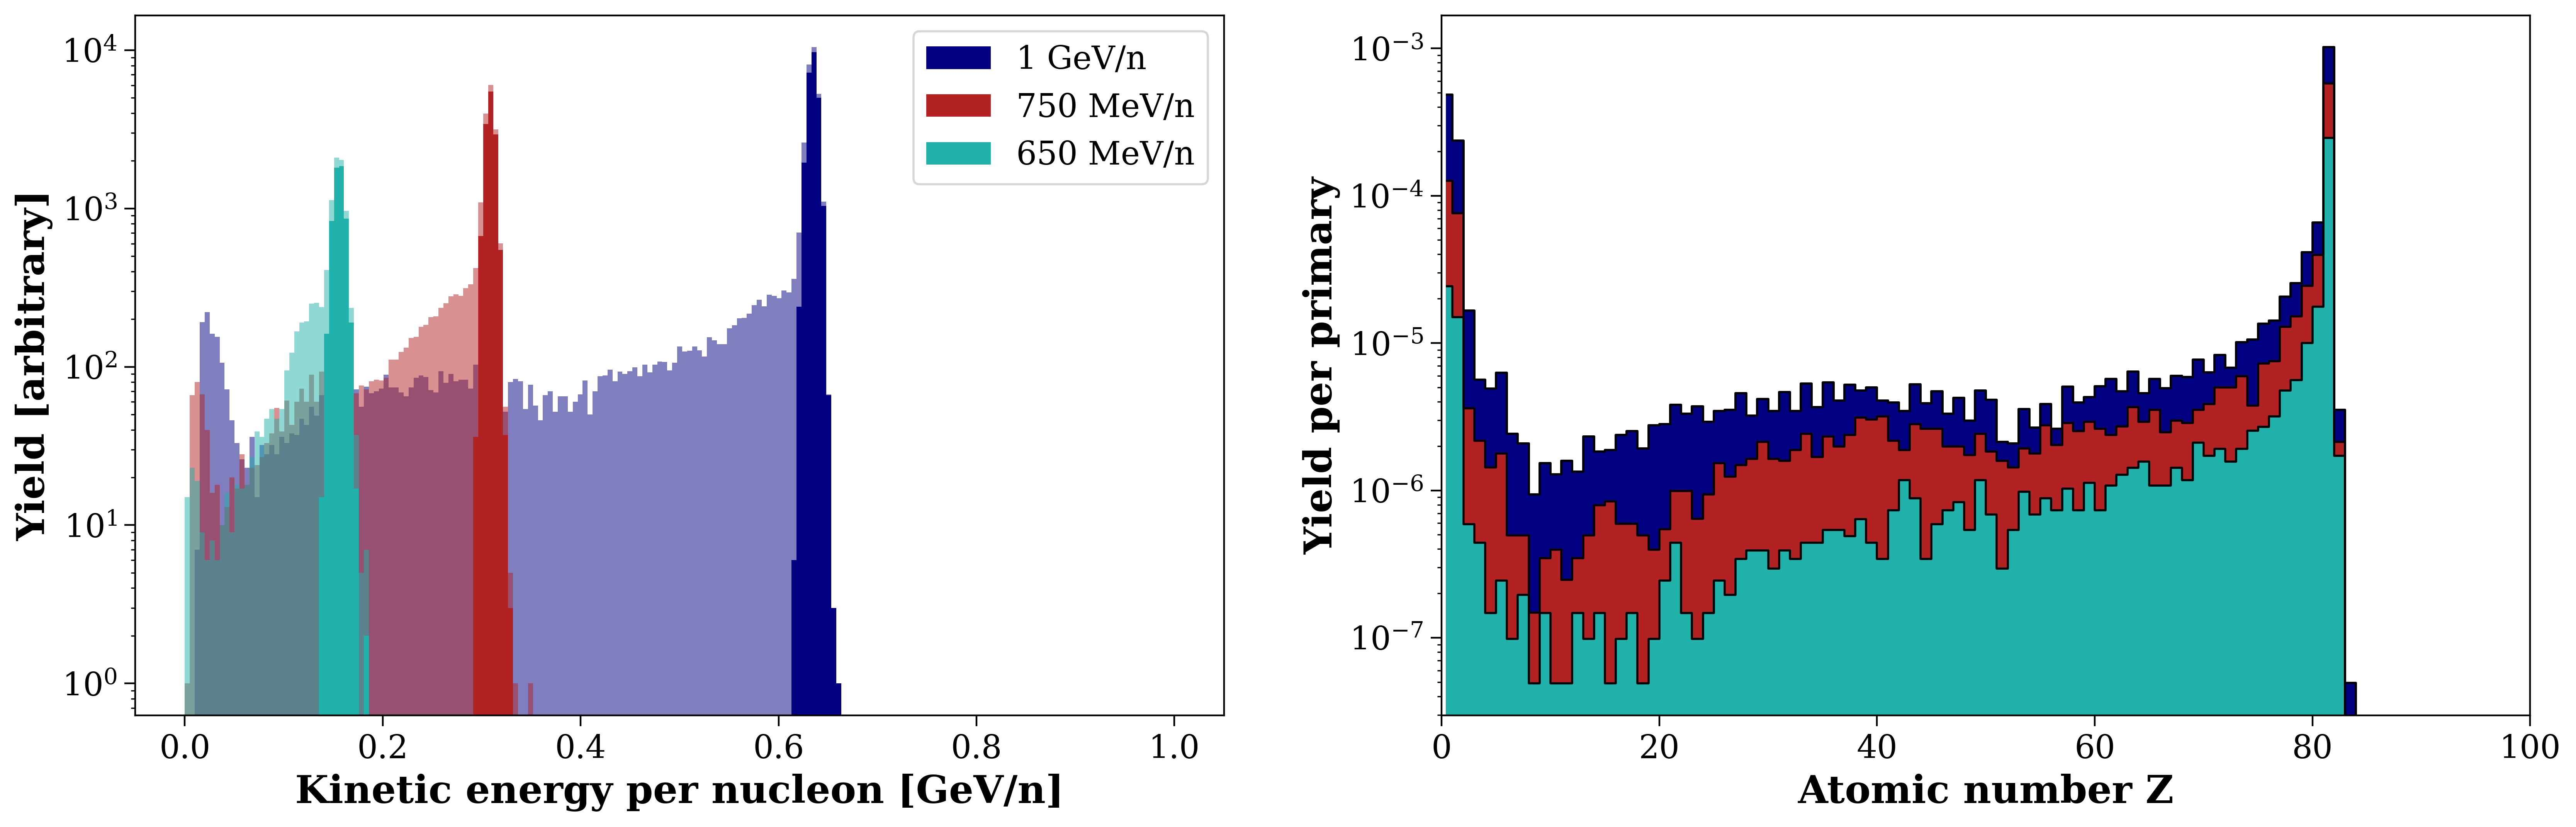
\includegraphics[width=\textwidth]{images/fragmentation.png}
    \vspace*{-0.5cm}
    \caption{FLUKA simulation results of the beam fragmentation for each of the energies used in the November 2022 experimental campaign, showing the resulting beam kinetic energy per nucleon distribution at the DUT (left) and the atomic number Z of each of the fragments (right).}
    \label{fig:fragmentation}
\end{figure}

\begin{figure}[t!]
    \centering
    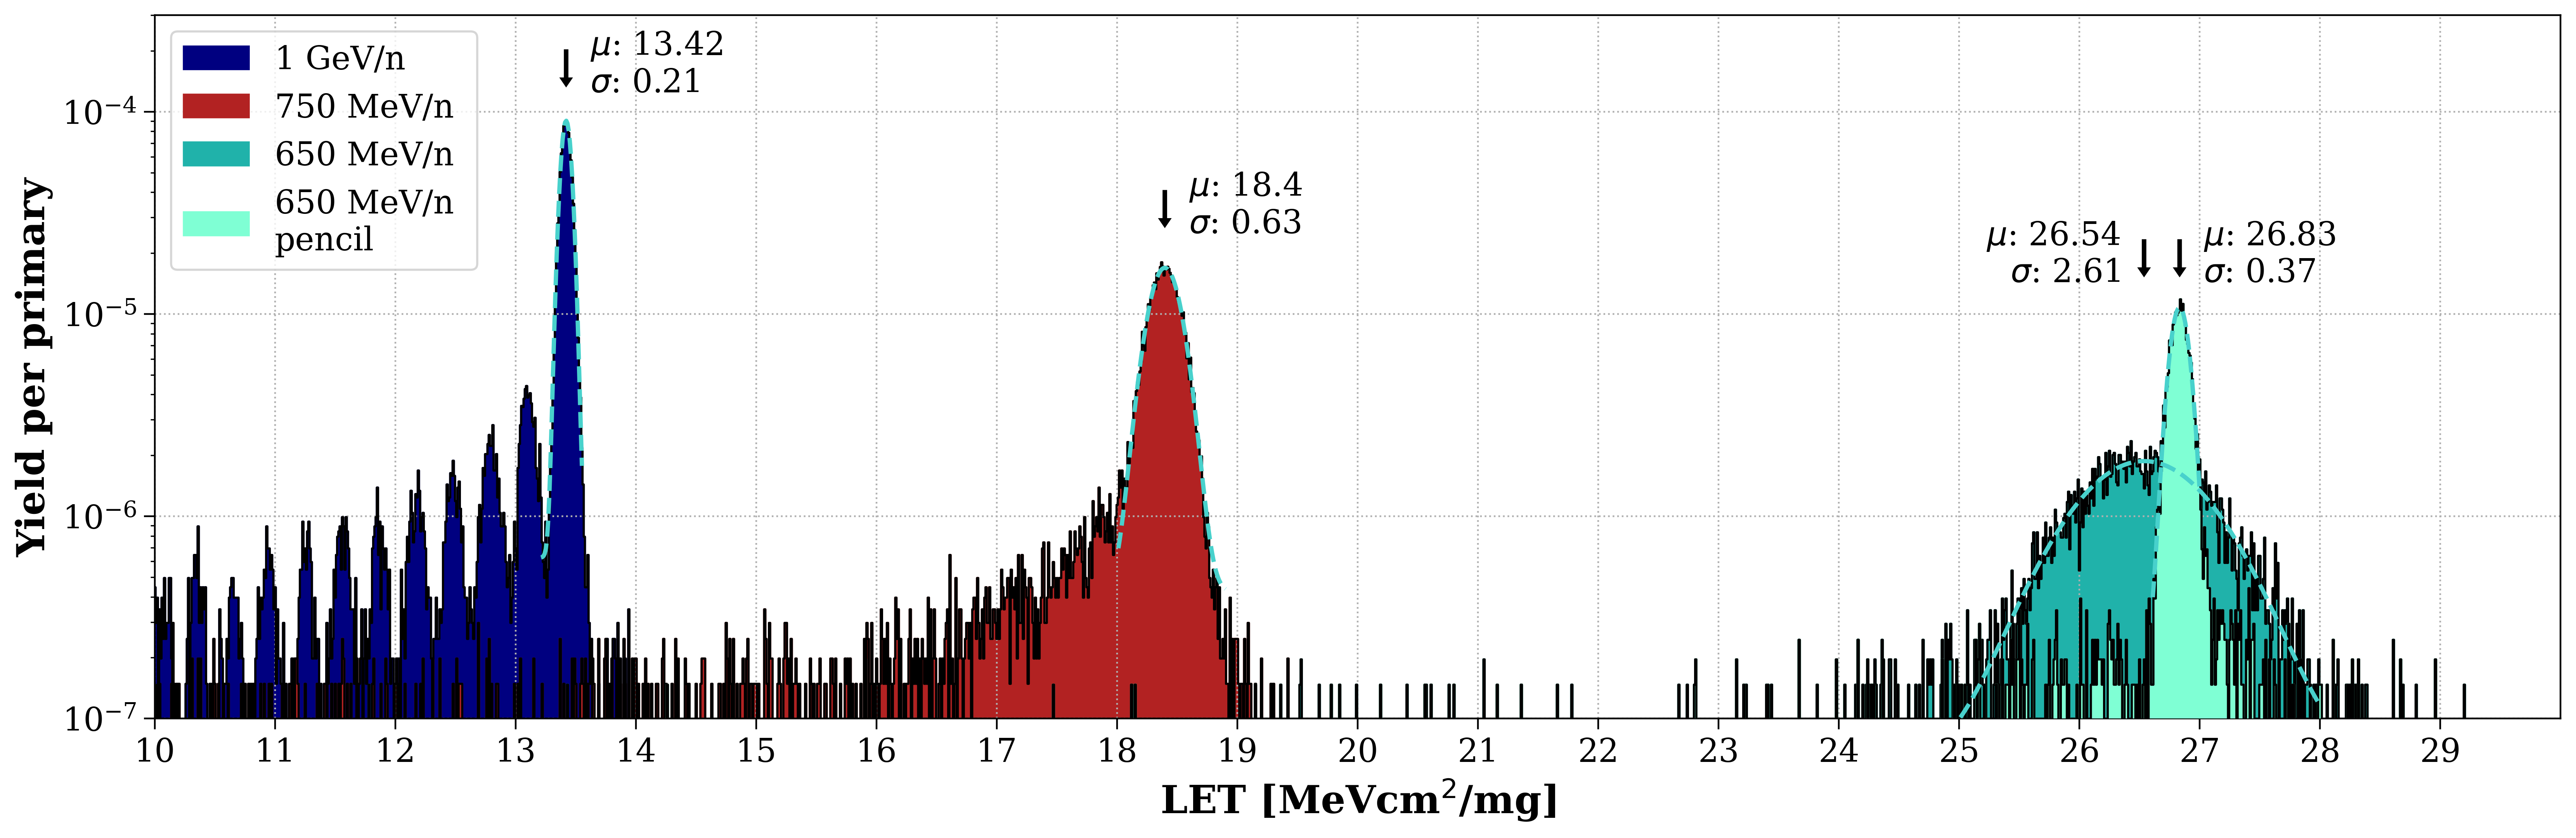
\includegraphics[width=\textwidth]{images/LETs.png}
    \vspace*{-0.5cm}
    \caption{FLUKA simulation results of the beam LET distribution at the DUT position for each of the energies used in the November 2022 experimental campaign. The primary peaks were fitted with a Gaussian to determine the parameters listed in Table \ref{tab:summary}. Note that in this plot the y-axis is in log scale, for this reason the FWHM of the primary peaks appears larger than it is.}
    \label{fig:LET}
\end{figure}